%!TEX TS-program = xelatex
%!TEX encoding = UTF-8 Unicode
% !Mode:: "TeX:UTF-8"

\documentclass[a4paper,11pt, svgnames, oneside]{scrbook} %如果不加oneside,则奇偶页的边距会不同,以方便装订
\usepackage[a4paper, top=2cm, bottom=2cm, left=2cm, right=2cm]{geometry}
\usepackage{ulem} %下划线,强调处理
\usepackage{ xunicode, xltxtra, fancybox, setspace,xcolor}

\usepackage{fontspec}
%\defaultfontfeatures{Mapping=tex-text,Scale=MatchLowercase} 
\setmainfont{DejaVu Serif} 
\setsansfont{DejaVu Sans} 
\setmonofont{DejaVu Sans Mono} 

\usepackage[CJKmath=true,CJKchecksingle]{xeCJK}
%\xeCJKsetup{AutoFakeBold=true, AutoFakeSlant=true} 
\setCJKmainfont[BoldFont={IPAGothic}]{FZLanTingHeiS-EL-GB} %方正字体,也可以改成:微软雅黑
\setCJKsansfont{FZLanTingHeiS-EL-GB} 
\setCJKmonofont{Ubuntu}


\usepackage{amsmath, amsthm, amsfonts, amssymb, mathrsfs} %数学公式相关 amssymb用于斜体字符,如varnothing,  masthm用于定理, mathrsfs用于花体字母
\newtheorem{theorem}{\hskip 2em \cjkem 定理}[chapter]
\newtheorem{lemma}{\hskip 2em \cjkem 引理}[chapter]
\newtheorem{proposition}{\hskip 2em \cjkem 命题} [chapter]
\newtheorem{example}{\hskip 2em \cjkem 例} [chapter]
\renewcommand{\proofname}{\hskip 2em \cjkem 证明}


\usepackage{caption, algorithm} %排版伪代码算法使用
\usepackage[]{algpseudocode}

\floatname{algorithm}{\cjkem{算法}}
\renewcommand{\algorithmicrequire}{\cjkem{输入:}} 
\renewcommand{\algorithmicensure}{\cjkem{输出:}}
\numberwithin{algorithm}{chapter}

\usepackage{colortbl, booktabs, multirow, makecell, longtable} %表格处理相关的Package

\usepackage{tikz, flowchart} % tikz绘图
\usepackage{pgfplots}
\usetikzlibrary{decorations.pathreplacing}
\usetikzlibrary{decorations.markings}
\usetikzlibrary{calc, arrows, arrows.meta, shapes, shadows, shapes.geometric, positioning}
\usetikzlibrary{topaths}
\usetikzlibrary{mindmap}
\usetikzlibrary{matrix}

\usepackage[tikz]{bclogo}  %see http://mirrors.ctan.org/graphics/bclogo/README
\DeclareGraphicsRule{.mps}{eps}{*}{} %解决xelatex处理bclogo时的mps问题
\newcommand{\infobox}[2]{ 
    \begin{bclogo}[couleur=yellow!10, logo=\bcfleur, ombre=true]{#1}
    #2
    \end{bclogo}
}
\newcommand{\warnbox}[2]{ 
    \begin{bclogo}[couleur=yellow!10, logo=\bctakecare, ombre=true]{#1}
    #2
    \end{bclogo}
}

\newcommand{\shellbox}[1]{ 
  \vspace{0.5cm}
  \begin{bclogo}[couleur=yellow!5, logo=\bccrayon, ombre=true]{命令}
    #1
  \end{bclogo}
}


\usepackage{listings}
\lstset{breakatwhitespace,
columns=fullflexible,
keepspaces=false,
breaklines,
keywordstyle=\color{blue},
extendedchars=true}


\lstset{breakatwhitespace,
backgroundcolor=\color{white},
columns=fullflexible,
breaklines,
showtabs=true,
tabsize=4,
keepspaces=true,
keywordstyle=\color{blue},
extendedchars=true}


% Definition of JavaScript
\definecolor{lightgray}{rgb}{.9,.9,.9}
\definecolor{darkgray}{rgb}{.4,.4,.4}
\definecolor{purple}{rgb}{0.65, 0.12, 0.82}

\lstdefinelanguage{JavaScript}{
  keywords={typeof, new, true, false, catch, function, return, null, catch, switch, var, if, in, while, do, else, case, break},
  keywordstyle=\color{blue}\bfseries,
  ndkeywords={class, export, boolean, throw, implements, import, this},
  ndkeywordstyle=\color{darkgray}\bfseries,
  identifierstyle=\color{black},
  sensitive=false,
  comment=[l]{//},
  morecomment=[s]{/*}{*/},
  commentstyle=\color{purple}\ttfamily,
  stringstyle=\color{red}\ttfamily,
  morestring=[b]',
  morestring=[b]"
}

\lstset{
   language=JavaScript,
   %backgroundcolor=\color{lightgray},
   extendedchars=true,
   basicstyle=\footnotesize\ttfamily,
   showstringspaces=false,
   showspaces=false,
   numbers=left,
   numberstyle=\footnotesize,
   numbersep=9pt,
   tabsize=2,
   breaklines=true,
   showtabs=false,
   captionpos=t
}


% Definition of CSS
\definecolor{lightgray}{rgb}{0.95, 0.95, 0.95}
\definecolor{darkgray}{rgb}{0.4, 0.4, 0.4}
\definecolor{purple}{rgb}{0.65, 0.12, 0.82}

\lstdefinelanguage{CSS}{
    keywords={color,background-image,margin,padding,font,weight,display,position,top,left,right,bottom,list,style,border,size,white,space,min,width, transform, transition, transition-property, transition-duration, transition-timing-function},
    alsodigit={-},
    sensitive=true,
    morecomment=[l]{//},
    morecomment=[s]{/*}{*/},
    morestring=[b]',
    morestring=[b]"
}

\lstset{%
    % General design
    %backgroundcolor=\color{lightgray},
    basicstyle={\small\ttfamily},   
    frame=l,
    % Code design
    identifierstyle=\color{black},
    keywordstyle=\color{blue}\bfseries,
    ndkeywordstyle=\color{greenCode}\bfseries,
    stringstyle=\color{ocherCode}\ttfamily,
    commentstyle=\color{darkgray}\ttfamily,
    % Code
    language={CSS},
    tabsize=2,
    showtabs=false,
    showspaces=false,
    showstringspaces=false,
    extendedchars=true,
    breaklines=true,
    % line-numbers
    xleftmargin={0.75cm},
    numbers=left,
    stepnumber=1,
    firstnumber=1,
    numberfirstline=true,
}


\definecolor{orangered}{RGB}{239,134,64}
\definecolor{tagcolor}{RGB}{0,0,150}
\definecolor{keywordcolor}{RGB}{139,38,201}
\definecolor{attr_value_color}{RGB}{153,51,0}

\lstset{
    language=XML,
    tabsize=4,
    %caption=Code,
    label=code:sample,
    frame=shadowbox,
    rulesepcolor=\color{gray},
    xleftmargin=20pt,
    framexleftmargin=15pt,
    keywordstyle=\color{keywordcolor}\bf,
    commentstyle=\color{gray},
    stringstyle=\color{attr_value_color},    
    tagstyle=\color{tagcolor}\bf,
    markfirstintag=\color{red}\bf,
    numbers=left,
    numberstyle=\tiny,
    numbersep=5pt,
    breaklines=true,
    showstringspaces=false,
    basicstyle=\footnotesize,
    morekeywords={xmlns,version,type,encoding,xml-stylesheet, xs:schema,xs:element,xs:complexType,xs:sequence,xs:attribute}, % list your attributes here
    emphstyle={\color{blue}}}
\renewcommand{\lstlistingname}{Code}



\usepackage{indentfirst}  %首行缩进
\setlength{\parindent}{2em} 
\setlength{\listparindent}{2em} %item列表的段落缩进量
\usepackage{enumitem}
\setenumerate[1]{itemsep=0pt,partopsep=0pt,parsep=\parskip,topsep=5pt}
\setitemize[1]{itemsep=0pt,partopsep=0pt,parsep=\parskip,topsep=5pt}

\usepackage{fancyhdr}
\thispagestyle{empty}

% 设置 plain style 的属性
\fancypagestyle{plain}{%
		\fancyhf{} % 清空当前设置

		% 设置页眉 (head)
		\fancyhead[RE]{\leftmark} % 在偶数页的右侧显示章名
		\fancyhead[LO]{\rightmark} % 在奇数页的左侧显示小节名
		\fancyhead[LE,RO]{~\thepage~} % 在偶数页的左侧,奇数页的右侧显示页码

		% 设置页脚:在每页的右下脚以斜体显示书名
		%\fancyfoot[RO,RE]{ {\it Written by Summer XIA}, Email: {\it xiat@ruc.edu.cn}}

		\renewcommand{\headrulewidth}{0.7pt} % 页眉与正文之间的水平线粗细
		\renewcommand{\footrulewidth}{0pt}
}

\pagestyle{fancy} % 选用 fancy style
% 其余同 plain style
\fancyhf{}
\fancyhead[RE]{\leftmark}
\fancyhead[LO]{\rightmark}
\fancyhead[LE,RO]{~\thepage~}
%\fancyfoot[RO,RE]{{\it Written by  Summer XIA}, Email: {\it xiat@ruc.edu.cn}}


%%%%%%%%%% 一些重定义 %%%%%%%%%%
\renewcommand{\contentsname}{目录}     % 将Contents改为目录
\renewcommand{\indexname}{索引}
\renewcommand{\figurename}{图}
\renewcommand{\tablename}{表}
\renewcommand{\appendixname}{附录}

\renewcommand{\bibname}{参考文献}
\let\oldbibliography\thebibliography
\renewcommand\thebibliography[1]{
	\oldbibliography{#1}
	\setlength{\parskip}{0pt}
	\setlength{\itemsep}{0pt plus 0.2ex}
}

\newcommand{\tab}{\phantom{o}\hspace{2ex}}


\usepackage{draftwatermark}
\SetWatermarkText{}%设置水印文字
\SetWatermarkLightness{0.9}%设置水印亮度
\SetWatermarkScale{0.5}%设置水印大小

\usepackage{hyperref} %url引用

\usepackage{kpfonts}
\usepackage[bf, explicit]{titlesec} %对标题的式样进行设置
\newcommand*\chapterlabel{}
\titlespacing*{\chapter}{0pt}{50pt}{-60pt}
\renewcommand{\chaptername}{}
\titleformat{\section}[hang]{\color{MidnightBlue}\LARGE\bfseries}{\color{MidnightBlue}{\thesection} }{.8em}{#1}
\titleformat{\subsection}[hang]{\color{NavyBlue}\Large\bfseries}{\color{NavyBlue}{\thesubsection} }{.8em}{#1}
\titleformat{\subsubsection}[hang]{\large\bfseries}{\thesubsection}{.8em}{\hspace{1em} $\blacksquare$ \cjkem #1}


%自定义的一些命令,方便使用
\newcommand*\circled[1]{\tikz[baseline=(char.base)]{
  \node[shape=circle,draw,inner sep=1.5pt] (char) {#1};}}


%\newcommand*{\hei}{\fontfamily{FZLanTingHeiS-H-GB}\selectfont}
%\DeclareTextFontCommand{\texthei}{\hei}

\setCJKfamilyfont{FZHei}{FZLanTingHeiS-R-GB}  
\newcommand{\cjkbold}{\color[rgb]{0.29, 0.0, 0.51} \CJKfamily{FZHei}}  %http://latexcolor.com/

\setCJKfamilyfont{FZHeiR}{FZLanTingHeiS-R-GB}  
\newcommand{\cjkem}{\CJKfamily{FZHeiR}} 

\begin{document}

    \frontmatter

    
\titleformat{\chapter}
  {\gdef\chapterlabel{}
   \normalfont\sffamily\Huge\bfseries\scshape}
  {\gdef\chapterlabel{\thechapter\ }}{0pt}
  {
	\begin{tikzpicture}[remember picture,overlay]
	\node[yshift=-4cm] at (current page.north west)
	  {\begin{tikzpicture}[remember picture, overlay]
		\draw[fill=LightSkyBlue!20, draw=black, dashed] (0,0) rectangle
		  (\paperwidth,4cm);
		\node[anchor=east,xshift=.9\paperwidth,rectangle,
			  rounded corners=20pt,inner sep=11pt,draw,
			  fill=white, minimum width=6cm](name)
			  {  {\chapterlabel} \color{black}  #1   };
	   \end{tikzpicture}
	  };
   \end{tikzpicture}
   \vspace{2em}
  }




\usetikzlibrary{calc}
\title{
    \huge{\textcolor{blue}{Python 3与数据分析基础 \\---数据科学家的分析利器}} \\ ~ \\
	\begin{tikzpicture}
	\node[fill=green!60, shading=ball, ball color=red!90, shape=circle, inner sep=0.5cm] (0) {};
	\foreach \angle/\index in {0/1,60/2,120/3,180/4, 240/5, 300/6}{
		\node[fill=blue!60, shading=ball, ball color=blue!75, shape=circle, inner sep=0.4cm] (\index) at (\angle:4) {};
		\draw[line width=0.1cm, draw=blue!50] (0) to (\index);
	};
	\foreach \angle/\index in {30/1,90/2,150/3,210/4, 270/5, 330/6}{
		\node[fill=blue!60, shading=ball, ball color=green!80, shape=circle, inner sep=0.3cm] (\index) at (\angle:2.4) {};
		\draw[line width=0.1cm, draw=green!70] (0) to (\index);
	};
	\end{tikzpicture}
}
\author{
    夏天@IRM-Renmin University of China 
}

% General definitions for all Chapters
%-------------------------------------------------------------------------------
% Define Page style for all chapters


% Set double spacing for the text
\doublespacing
%-------------------------------------------------------------------------------


% 1st page for the Title
%-------------------------------------------------------------------------------
\maketitle

%-------------------------------------------------------------------------------
%用于生成罗马计数的前言
\frontmatter


       % include title page
    \chapter*{序言}

Python 是一门简单易学、功能强大的编程语言。它具有高效的高级数据结构和简单而有效的面向对象编程的特性。Python 优雅的语法和动态类型、 以及其解释性的性质,使它在许多领域和大多数平台成为脚本编写和快速应用程序开发的理想语言。

从 Python 网站 https://www.python.org/可以免费获得所有主要平台的源代码或二进制形式的Python 解释器和广泛的标准库,并且可以自由地分发。网站还包含许多免费的第三方 Python 模块、 程序、工具以及附加文档的发布包和链接。

Python 解释器可以用 C 或 C+ +  (或调用C的其他语言)中轻松的对新的函数和数据类型进行扩展Python 也适合作为可定制应用程序的一种扩展语言。

本教程通俗地向读者介绍 Python 语言及其体系的基本概念和功能。 随手使用Python 解释器来亲自动手实践是很有帮助的,并且由于所有示例都是自成体系的,所以本教程也可以离线阅读。

有关标准对象和模块的说明,请参阅Python 标准库。 Python语言参考 给出了Python语言的更正式的定义。要编写 C 或 C+ + 的扩展,请阅读扩展和嵌入Python解释器 与Python/C API参考手册。也有几本书深度地介绍了Python 。

本教程不会尝试全面地涵盖每一个单独特性,甚至即使它是常用的特性。相反,它介绍了许多 Python 的值得注意的特性,从而能让你很好的把握这门语言的特性。经过学习,你将能够阅读和编写Python 的模块和程序,并可以更好的学会 Python 标准库 中描述的各种 Python 库模块。


\subsection*{图书网站和相关资源}

本书的网站和附带资源可以通过以下网址获得:

\url{http://dmml.asu.edu/smm}

网站同时提供了配套课件、练习题和示范工程,同时给出了与社会媒体挖掘相关的公共资源入口。

\subsection*{教师须知}

本书按照高年级本科生或研究生一个学期的学习课程进行设计,主要面向拥有计算机科学背景的学生,但对于掌握概率论、统计和线性代数基础知识的读者,也很容易理解本书内容。本书部分章节用于回顾一些基础知识,学生已掌握该部分内容时可忽略这些章节。例如,如果学生已经学过了数据挖掘或机器学习课程,可略过第5章。如果时间受限,第6章至第8章应深入讨论,但第9章和第10章可以简要讨论或者作为阅读材料部分。

~\\
~\\
~\\

\begin{flushright}
\emph{
	Reza Zafarani \\
	Mohammad Ali Abbasi \\
	Huan Liu
}

2013年8月于美国 亚利桑那州 坦佩
\end{flushright}





       % include preface
    %generate book content list
\setcounter{tocdepth}{6}
\tableofcontents
       % include content

    %\include{other}         % include other frontmatter
  

    \mainmatter


			\titleformat{\chapter}
			  {\gdef\chapterlabel{}
			   \normalfont\sffamily\Huge\bfseries\scshape}
			  {\gdef\chapterlabel{\thechapter\ }}{0pt}
			  {
				\begin{tikzpicture}[remember picture,overlay]
				\node[yshift=-5cm] at (current page.north west)
				  {\begin{tikzpicture}[remember picture, overlay]
					\draw[fill=orange!20, draw=black, dotted] (0,0) rectangle
					  (\paperwidth,5cm);
					\node[scale=1.3, rounded corners=5pt, line width=2pt, dotted, draw=orange!80, minimum width=2cm, minimum height=2cm] at (3.5,2.5) {  \color{orange}~$\chapterlabel$ $\hookleftarrow$  };
					\node[anchor=east,xshift=.9\paperwidth,rectangle,
						  rounded corners=20pt,inner sep=11pt,draw,
						  fill=white, minimum width=7cm](name)
						  {\color{black} 第 \chapterlabel 章~~  #1 };
				   \end{tikzpicture}
				  };
			   \end{tikzpicture}
				\vspace{4em}
			  }

     
     \begin{frame}[fragile]{整体内容}
  \begin{easylist} \easyitem
    & 简介
    & 数据类型
    & 控制流
    & 函数
    & 模块
    & 标准库
    & 面向对象编程
    & 异常、调试与测试
    & 输入输出
    & 应用(Web, DB, etc.)
  \end{easylist}
\end{frame}


\begin{frame}[fragile]{致谢}
  \begin{easylist}
    & 本课件的制作参考了部分图书和第三方网络资源,在此对原作者表达致谢和敬意,如
    有侵权需要从本课件中移除,请留言或联系xiat(at)ruc.edu.cn。参考资料包括但不限
    于以下:
    && 廖雪峰,
    \href{http://www.liaoxuefeng.com/wiki/0014316089557264a6b348958f449949df42a6d3a2e542c000}{Python教程}
    && Introducing Python by Bill Lubanovic
    && Dive Into Python 3 by Mark Pilgrim
    && Magnus Lie Hetland, 司维等翻译,Python基础教程(2ed), 人民邮电出版社
    && NumPy Cookbook
    && Python for Data Analysis
  \end{easylist}

\end{frame}

\section{引论}

\begin{frame}[fragile]{CH1 简介}
  \begin{easylist} \easyitem
    & 1.1 什么是Python
    & 1.2 Python可以做什么
    & 1.3 如何安装Python
    & 1.4 Python开发环境
    & 1.5 如何运行Python程序
    & 1.6 若干例子
  \end{easylist}
\end{frame}

\begin{frame}[fragile]{You're flying!}
  \begin{center}
    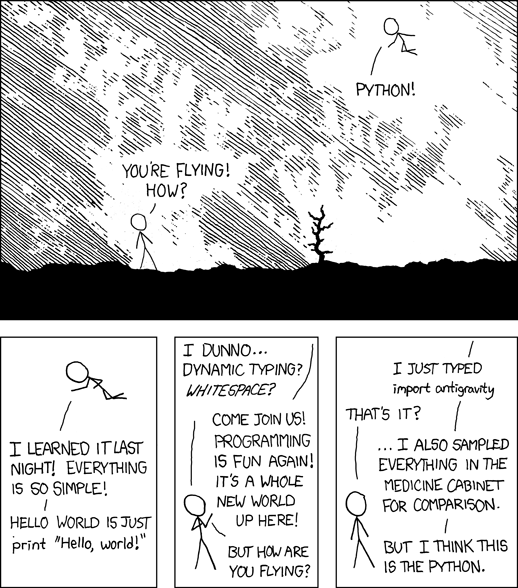
\includegraphics[height=0.9\textheight]{figure/fly.jpg}
  \end{center}
\end{frame}

\begin{frame}[fragile]{用Python,飞一般的感觉!}
  \begin{easylist}
    & \color{red} Friend :“你在飞!怎么做到的?”
    & Cueball:“Python!我昨晚刚刚学会了Python。一切都变得如此简单!写一个Hello World 程序只要一行代码 print "Hello World!" 就搞定了!”
    & \color{red}Friend :“ 什么情况?呃……动态类型?泛空格符?”
    & Cueball:“来加入我们吧,有了Python,编程再次变得有趣。这是一个全新的世界!”
    & \color{red}Friend :“但是你到底是怎么飞在天上的?”
    & Cueball:“我只是输入了“import antigravity” 命令而已。”
    & \color{red}Friend :“就这样?”
    & Cueball:“我还把药柜中的药嗑了个遍……但我觉得还是 Python 的原因。”
  \end{easylist}
\end{frame}

\begin{frame}[fragile]{1.1 什么是Python}
  \begin{easylist}
    & Python是一种既简单又强大的编程语言
    & 注重如何解决问题,而不是编程语言的语法和结构
    & 拥有高效的高级数据结构,简单有效地实现面向对象编程
    & 语法简洁、动态解释、适用于快速应用开发和脚本编程
    & 在数据科学中大有用武之地
  \end{easylist}
\end{frame}

\begin{frame}[plain]{}
  \begin{tikzpicture}[remember picture,overlay]
    \node[xshift=-60, yshift=-60] at (current page.north east) {
\includegraphics[]{figure/tim.png} };
  \end{tikzpicture}

  \LARGE The Zen of Python, \small by Tim Peters

  \normalsize 
  Beautiful is better than ugly. \\
  Explicit is better than implicit. \\
  Simple is better than complex. \\
  Complex is better than complicated. \\
  Flat is better than nested. \\
  Sparse is better than dense. \\
  Readability counts. \\
  Special cases aren't special enough to break the rules. \\
  Although practicality beats purity. \\
  Errors should never pass silently. \\
  Unless explicitly silenced.\\
  In the face of ambiguity, refuse the temptation to guess.\\
  There should be one-- and preferably only one --obvious way to do it.\\
  Although that way may not be obvious at first unless you're Dutch.\\
  Now is better than never.\\
  Although never is often better than *right* now.\\
  If the implementation is hard to explain, it's a bad idea.\\
  If the implementation is easy to explain, it may be a good idea.\\
  Namespaces are one honking great idea -- let's do more of those!\\
\end{frame}

\begin{frame}[plain]{}
  \begin{tikzpicture}[remember picture,overlay]
    \node[xshift=-60, yshift=-60] at (current page.north east) {
\includegraphics[]{figure/tim.png} };
  \end{tikzpicture}

  \LARGE Python之禅 \small by Tim Peters

  \normalsize
  优美胜于丑陋 \\ {\tiny Python 以编写优美的代码为目标}\\
  明了胜于晦涩 \\ {\tiny 优美的代码应当是明了的,命名规范,风格相似}\\
  简洁胜于复杂 \\ {\tiny 优美的代码应当是简洁的,不要有复杂的内部实现}\\
  复杂胜于凌乱 \\ {\tiny 如果复杂不可避免,那代码间也不能有难懂的关系,要保持接口简洁}\\
  扁平胜于嵌套 \\ {\tiny 优美的代码应当是扁平的,不能有太多的嵌套}\\
  间隔胜于紧凑 \\ {\tiny 优美的代码有适当的间隔,不要奢望一行代码解决问题}\\
  可读性很重要 \\ {\tiny 优美的代码是可读的}\\
  即便假借特例的实用性之名,也不可违背这些规则 \\ {\tiny 这些规则至高无上} \\
  不要包容所有错误,除非你确定需要这样做 \\ {\tiny 精准地捕获异常,不写 except:pass 风格的代码}\\
  当存在多种可能,不要尝试去猜测\\
  而是尽量找一种,最好是唯一一种明显的解决方案({\tiny 如果不确定,就用穷举法})\\
  虽然这并不容易,因为你不是 Python 之父({\tiny 这里的 Dutch 是指 Guido})\\
  做也许好过不做,但不假思索就动手还不如不做({\tiny 动手之前要细思量})\\
  如果你无法向人描述你的方案,那肯定不是一个好方案;反之亦然(方案测评标准)\\
  命名空间是一种绝妙的理念,我们应当多加利用(倡导与号召)\\
\end{frame}

\begin{frame}[fragile]{编程语言排名@Feb, 2016}
  \begin{easylist}
    & Java
    & C
    & C++
    & C\#
    & \em Python $\star$
    & PHP
    & Visual Basic
    & Perl
    & JavaScript
    & Delphi/Object Pascal
  \end{easylist}
  From: \url{http://www.tiobe.com/tiobe_index?page=index}
\end{frame}


\begin{frame}[fragile]{1.2 Python可以做什么}
  \begin{easylist}
    & Almost anything
    && From system management, security, web, \\
    to data mining, machine learning ...
    & 数据科学界华山论剑:R与Python巅峰对决 \\
    \url{http://chuansong.me/n/1458679}
    & 为什么很多人喜欢 Python? \\
    \url{https://www.zhihu.com/question/28676107}
  \end{easylist}
\end{frame}

\begin{frame}[fragile]{一段简单的Python代码}
~
  \begin{python}
    #Python 3: Fibonacci series up to n
    def fib(n):
        a, b = 0, 1
        while a < n:
            print(a, end=', ')
            a, b = b, a+b
        print()
    fib(100)
  \end{python}
  Result: 0, 1, 1, 2, 3, 5, 8, 13, 21, 34, 55, 89, 

\end{frame}


\begin{frame}[fragile]{1.3 如何安装Python}
  \begin{easylist}
    & 在线直接编写运行
    && Host, run, and code Python in the cloud!
    && https://www.python.org/
    & python shell及增强版本
    & 编辑器编辑代码文件,利用python运行
  \end{easylist}
\end{frame}

\begin{frame}[fragile]{Python shell}
  \begin{bash}
    $python3
    Python 3.4.3+ (default, Oct 14 2015, 16:03:50) 
    [GCC 5.2.1 20151010] on linux
    Type "help", "copyright", "credits" or "license" for more information.
    >>> 
  \end{bash}
\end{frame}

\begin{frame}[fragile]{课堂练习}
  \begin{easylist}
    & Windows环境下Python程序的安装和运行测试
    && https://www.python.org/downloads/
    & 注意:本课程后续讲解均以Linux(Ubuntu)作为操作系统环境
  \end{easylist}
\end{frame}

\begin{frame}[fragile]{安装EasyInstall}
  \begin{easylist}
    & wget\textvisiblespace http://peak.telecommunity.com/dist/ez\_setup.py
    & python\textvisiblespace ez\_setup.py\textvisiblespace setuptools
    & ez\_install\textvisiblespace pip
    & ez\_install\textvisiblespace pip3
  \end{easylist}
\end{frame}

\begin{frame}[fragile]{Python2 vs Python3}
  \begin{easylist}
    & Python3是Python2的重大变更版本
    & 有许多正在运行的程序使用了Python2
    & 系统中可以同时安装python2和python3
    & 与Python2相比,Python3相关的工具多以3结尾,如ipython3
    & 本课程讲解以Python3为主,穿插Python2的语法
  \end{easylist}
\end{frame}


\begin{frame}[fragile]{1.4 Python开发环境}
  \begin{easylist}
    & Python shell
    && 自带的命令解释器
    && ipython
    && jupyter notebook
    && bpython
    & Editor
    && pycharm
    && Sublime text
    && Emacs
    && Vim
  \end{easylist}
\end{frame}

\begin{frame}[fragile]{ipython}
  \begin{easylist}
    & sudo\textvisiblespace apt-get\textvisiblespace install\textvisiblespace ipython3
    & 展示
  \end{easylist}
\end{frame}

\begin{frame}[fragile]{bpython}
  \begin{easylist}
    & sudo\textvisiblespace apt-get\textvisiblespace instal\textvisiblespace bpython3
    & 展示
  \end{easylist}
\end{frame}

\begin{frame}[fragile]{善用help}
  利用Python自带的help函数获取帮助

  \pyinline{help(max)}

  \pyinline{help()}
\end{frame}

\begin{frame}[fragile]{增强命令行}
  \begin{easylist}
    & tmux
    & zsh
  \end{easylist}
\end{frame}


\begin{frame}[fragile]{1.5 如何运行Python程序}
  \begin{easylist}
    & 直接在Python Shell中输入,解释执行
    & 保存到文件中,以.py结尾,通过python运行
    && 如把前面的斐波那契数列的代码保存到文本文件中,并把文件名命名为fib.py
    && python3\textvisiblespace fib.py
    \pause
    & 可执行的Python脚本
    && 在Python脚本文件的开头加上一行声明 
    &&& \#!/usr/bin/python3
    &&& chmod u+x filename.py
  \end{easylist}
\end{frame}

\begin{frame}[fragile]{代码清单:fib.py}
  \lstinputlisting[keywordstyle=\ttfamily]{src/fib.py}
\end{frame}

\begin{frame}[fragile, allowframebreaks]{1.6 一个完整的Python程序}
  \lstinputlisting[keywordstyle=\ttfamily, basicstyle=\rmfamily\normalsize]{src/humansize.py}
  Code From: ``Dive into Python 3''
\end{frame}

\begin{frame}[fragile]{例子解释}
  \begin{easylist}
    & 如何声明函数:def
    & 可选的和命名的参数
    & 文档字符串
    & 代码缩进
    & 异常
    & 大小写  
  \end{easylist}
\end{frame}

\begin{frame}[fragile]{Python基本用法预览}
  \begin{easylist}
    & 把Python当做计算器
    & 字符串的表示
    & 字符串切片
  \end{easylist}
\end{frame}

\begin{frame}[fragile]{把Python当做计算器}
  \begin{easylist}
    & Python解释器可以当做简单的计算器,输入表达式,即可对表达式求值
    & 练习
    && 打开Python解释器,输入以下表达式求值
    && 2+2
    && 8/5 \#结果是1.6? 还是1? %默认不会丢失小数部分
    && (3+5)/2
    && 8//5 %相当于整除 
  \end{easylist}
\end{frame}

\begin{frame}[fragile]{字符串的表示}
  \begin{easylist}
    & 单引号
    & 双引号
    & 三引号
  \end{easylist}
  \begin{python}
    msg = 'hello "Python"'
    print(msg)
    msg = "hello 'Python'"
    print(msg)
    msg = '''
        hello
        world!
        '''
    print(msg)
  \end{python}
\end{frame}


\begin{frame}[fragile]{字符串切片}
    $>>>$ msg = '中国人民大学信息资源管理学院'

    $>>>$ msg[0] \\ '中'

    $>>>$ msg[-8:-1] \\ '信息资源管理学'

    $>>>$ ms g[-8:] \\ ??

    $>>>$ msg[:6] 

    $>>>$ msg[:]
\end{frame}


\begin{frame}[fragile]{---END---}
  \begin{center}
    \Simley{1}{10}{1}
  \end{center}
\end{frame}

%%% Local Variables:
%%% mode: latex
%%% TeX-master: "../python"
%%% End:

     %\part{基础知识}
     %\include{chapter/graph_essentials}
     
    \appendix
    %\include{history}       % include first appendix
    %\include{tables}        % include second appendix, etc.
    
    
	\backmatter

		\titleformat{\chapter}
		  {\gdef\chapterlabel{}
		   \normalfont\sffamily\Huge\bfseries\scshape}
		  {\gdef\chapterlabel{\thechapter\ }}{0pt}
		  {
			\begin{tikzpicture}[remember picture,overlay]
			\node[yshift=-4cm] at (current page.north west)
			  {\begin{tikzpicture}[remember picture, overlay]
				\draw[fill=LightSkyBlue!20, draw=black, dashed] (0,0) rectangle
				  (\paperwidth,4cm);
				\node[anchor=east,xshift=.9\paperwidth,rectangle,
					  rounded corners=20pt,inner sep=11pt,draw,
					  fill=white, minimum width=6cm](name)
					  {  {\chapterlabel} \color{black}  #1   };
			   \end{tikzpicture}
			  };
		   \end{tikzpicture}
			\vspace{2em}
		  }
	
	\bibliographystyle{plain}
	%\bibliography{bibliography}
    %\begin{thebibliography}{999}
\bibitem {MAA2012} Mohammad Ali Abbasi, Sun-Ki Chai, Huan Liu, and Kiran. Sagoo, Real-world behavior analysis through a social media lens., Social Computing, Behavioral-Cultural Modeling and Prediction, Springer, 2012, pp. 18–26.

\bibitem {Abello2002} J. Abello, M. Resende, and S. Sudarsky, Massive quasi-clique detection., LATIN 2002: Theoretical Informatics (2002), 598–612.

\bibitem {Abrahamson1993} E. Abrahamson and L. Rosenkopf, Institutional and competitive band wagons: Using mathematical modeling as a tool to explore innovation diffusion., Academy of management review (1993), 487–517.

\bibitem {Adamic2003} L.A. Adamic and E. Adar, Friends and neighbors on the web., Social Networks 25 (2003), no. 3, 211–230.


\bibitem {Adomavicius2005} Gediminas Adomavicius and Alexander.Tuzhilin,Toward the nextgeneration of recommender systems: a survey of the state-of-the-art and possible extensions., IEEE Transactions on Knowledge and Data Engineering 17(2005), no.6, 734–749.

\bibitem {N. Agarwal2008} N. Agarwal, H. Liu, L. Tang, and P.S. Yu,Identifying the influential bloggers in a community, Proceedings of the International Conferenceon Web Search and Web Data Mining, ACM, 2008, pp. 207–218.

\bibitem {Orlin1995} R.K. Ahuja, T.L. Magnanti, J.B. Orlin, and K. Weihe, Network flows:theory, algorithms and applications., ZOR-Methods and Models of Operations Research 41 (1995), no. 3, 252–254.

\bibitem {Salem2006} [8] Mohammad Al Hasan, Vineet Chaoji, Saeed Salem, and Mohammed.Zaki, Link prediction using supervised learning., SDM’06: Workshop onLink Analysis, Counter-terrorism and Security, 2006.

\bibitem {Albert2000} R. Albert and A.L. Barab′asi, Topology of evolving networks: local eventsand universality., Physical review letters 85 (2000), no. 24, 5234–5237.

\bibitem {Anagnostopoulos2008} A. Anagnostopoulos, R. Kumar, and M. Mahdian, Influence and correlation in social networks, Proceedings of the 14th ACM SIGKD Dinternational conference on Knowledge Discovery and Data Mining,ACM, 2008, pp. 7–15.

\bibitem {Anderson1996} L.R. Anderson and C.A. Holt, Classroom games: information cascades.,The Journal of Economic Perspectives 10 (1996),no. 4, 187–193.

\bibitem {Charles1997} Lisa R. Anderson and Charles A. Holt , Information cascades in the laboratory., The American Economic Review (1997), 847–862.

\bibitem {Robert1992} Roy M Anderson, Robert M May, and B Anderson, Infectious diseasesof humans: dynamics and control., vol. 26, Wiley Online Library, 1992.

\bibitem {Ankerst1999} M. Ankerst, M.M. Breunig, H.P. Kriegel, and J. Sander, OPTICS:ordering points to identify the clustering structure., Proceedings of the 1999 ACM SIGMOD international conference on Management of Data (1999), 49–60.

\bibitem {Aral2009} S. Aral, L. Muchnik, and A. Sundararajan, Distinguishing influence-based contagion from homophily-driven diffusion in dynamic networks.,Proceedings of the National Academy of Sciences 106 (2009), no. 51,21544–21549.

\bibitem {Jaime2008} Jaime Arguello, Jonathan Elsas, Jamie Callan, and Jaime. Carbonell,Document representation and query expansion models for blog recommendation., Proceedings of the second international conference on Weblogs and Social Media (ICWSM), 2008.

\bibitem {Asch1956} S.E. Asch, Studies of independence and conformity: I. a minority of oneagainst a unanimous majority., Psychological Monographs: Generaland Applied 70 (1956), no. 9, 1–70.

\bibitem {Sitaram2010} Sitaram Asur and Bernardo A. Huberman, Predicting the future with social media. ieee international conference on, Web Intelligence and Intelligent Agent Technology, vol. 1, IEEE, 2010, pp. 492–499.

\bibitem {Backstrom2006} L. Backstrom, D. Huttenlocher, J.M. Kleinberg, and X. Lan, Groupformation in large social networks: membership, growth, and evolution,Proceedings of the 12th ACM SIGKDD international conference onKnowledge Discovery and Data Mining, ACM, 2006, pp. 44–54.

\bibitem {Marlow2010} L. Backstrom, E. Sun, and C. Marlow, Find me if you can: improving geographical prediction with social and spatial proximity., Proceedings of the 19th International conference on World Wide Web, ACM, 2010,pp. 61–70.

\bibitem {Bailey1975} N.T.J. Bailey, The mathematical theory of infectious diseases and its applications., Charles Griffin \& Company Ltd, 1975.

\bibitem {Bakshy2011} E. Bakshy, J.M. Hofman, W.A. Mason, and D.J. Watts, Everyone’s aninfluencer: quantifying influence on twitter, Proceedings of the fourth ACM international conference on Web Search and Data Mining,ACM, 2011, pp. 65–74.

\bibitem {Banerjee1992} A.V. Banerjee, A simple model of herd behavior., The Quarterly Journal of Economics 107 (1992), no. 3, 797–817.

\bibitem {Albert1999} A.L. Barab′asi and R. Albert, Emergence of scaling in random networks.,science 286 (1999), no. 5439, 509–512.

\bibitem {Gundech2013} Geoffrey Barbier, Zhuo Feng, Pritam Gundecha, and Huan. Liu, Morgan \& Claypool Publishers, 2013.

\bibitem {Gabriel2012} Geoffrey Barbier, Reza Zafarani, Huiji Gao, Gabriel Fung, and Huan.Liu, Maximizing benefits from crowd sourced data., Computational and Mathematical Organization Theory 18 (2012), no. 3, 257–279.

\bibitem {Barnes2004} S.J. Barnes and E. Scornavacca, Mobile marketing: the role of permissionand acceptance., International Journal of Mobile Communications 2(2004), no. 2, 128–139.

\bibitem {Alessandro2008} Alain Barrat, Marc Barthelemy, and Alessandro. Vespignani, Dynamical processes on complex networks., vol. 1, Cambridge UniversityPress, 2008.

\bibitem {Barwise2002} P. Barwise and C. Strong, Permission-based mobile advertising., Journal of Interactive Marketing 16 (2002), no. 1, 14–24.

\bibitem {Bass1969} F. Bass, A new product growth model for product diffusion., ManagementScience 15 (1969), 215–227.

\bibitem {Bell1924} W.G. Bell, The great plague in london in 1665., The Great Plague inLondon in 1665. (1924).

\bibitem {Bellma1956} R. Bellma, On a routing problem., NOTES 16 (1956), no. 1.

\bibitem {Bierlaire1998} M. Ben-Akiva, M. Bierlaire, H. Koutsopoulos, and R. Mishalani, Dy-namit: a simulation-based system for traffic prediction., DACCORS ShortTerm Forecasting Workshop, The Netherlands, 1998.

\bibitem {Berger2001} E. Berger, Dynamic monopolies of constant size., Journal of Combinatorial Theory, Series B 83 (2001), no. 2, 191–200.

\bibitem {Berkhin2006} P. Berkhin, A survey of clustering data mining techniques., Grouping Multidimensional Data (2006), no. c, 25–71.

\bibitem {Russell2012} H. Russell. Bernard, Social research methods: qualitative and quantitative approaches., Sage, 2012.

\bibitem {Bikhchandani1992} S. Bikhchandani, D. Hirshleifer, and I. Welch, A theory of fads, fashion, custom, and cultural change as informational cascades., Journal of Political Economy (1992), 992–1026.

\bibitem {Sharma2000} S. Bikhchandani and S. Sharma, Herd behavior in financial markets.,IMF Staff Papers (2000), 279–310.

\bibitem {Bishop1995} C.M. Bishop, Neural networks for pattern recognition., (1995).

\bibitem {Christopher2006} Christopher M. Bishop, Pattern recognition and machine learning., vol. 4, Springer,2006.

\bibitem {Bollob2001} B. Bollob′as, Random graphs., vol. 73, Cambridge University Press,2001.

\bibitem {Bonabeau1999} E. Bonabeau, M. Dorigo, and G. Theraulaz, Swarm intelligence: fromnatural to artificial systems., no. 1, Oxford University Press, 1999.

\bibitem {James2010} James Davidson, Benjamin Liebald, Junning Liu, Palash Nandy, Taylor Van Vleet, Ullas Gargi, Sujoy Gupta, Yu He, Mike Lambert, BlakeLivingston, and et al., The youtube video recommendation system., Proceedings of the fourth ACM conference on Recommender Systems,ACM, 2010, pp. 293–296.

\bibitem {Davies1979} D.L. Davies and D.W. Bouldin, A cluster separation measure., IEEE Transactions on Pattern Analysis and Machine Intelligence (1979),no. 2, 224–227.

\bibitem {Jarlais1994} D.C. Des Jarlais, S.R. Friedman, J.L. Sotheran, J. Wenston, M. Yan-covitz Marmor, Frank S.R., Beatrice B., and Mildvan D. S., Continuityand change within an hiv epidemic., JAMA: the journal of the American Medical Association 271 (1994), no. 2, 121–127.

\bibitem {Devenow1996} A. Devenow and I. Welch, Rational herding in financial economics.,European Economic Review 40 (1996), no. 3, 603–615.

\bibitem {Dia2001} H. Dia, An object-oriented neural network approach to short-term traffic forecasting., European Journal of Operational Research 131 (2001),no. 2, 253–261.

\bibitem {Diestel2005} R. Diestel, Graph theory. 2005., Graduate Texts in Math (2005).

\bibitem {Dietz1967} K. Dietz, Epidemics and rumours: a survey., Journal of the Royal Statistical Society. Series A (General) (1967), 505–528.

\bibitem {Dodds2004} P.S. Dodds and D.J. Watts, Universal behavior in a generalized model of contagion., Physical Review Letters 92 (2004), no. 21, 218701.

\bibitem {Drehmann2005} M. Drehmann, J. Oechssler, and A. Roider, Herding and contrarian behavior in financial markets – an internet experiment., (2005).

\bibitem {Richard2012} Richard O. Duda, Peter E. Hart, and David G. Stork, Pattern classification., Wiley-interscience, 2012.

\bibitem {Dunn1974} J.C. Dunn, Well-separated clusters and optimal fuzzy partitions., Journal of cybernetics 4 (1974), no. 1, 95–104.

\bibitem {Dye2003} C. Dye and N. Gay, Modeling the sars epidemic., Science 300 (2003),no. 5627, 1884–1885.

\bibitem {Nicholas2009} Nicholas A. Christakis and James H. Fowler, Connected: The surprising power of our social networks and how they shape our lives., Norskepidemiologi= Norwegian Journal of Epidemiology 19 (2009), no. 1,5.

\bibitem {Chung1997} F.R.K. Chung, Spectral graph theory., no. 92, American Mathematical Society, 1997.

\bibitem {Cialdini1998} R. B. Cialdini and M. R. Trost., Social influence: Social norms, conformity and compliance., (1998), 151.

\bibitem {Aaron2009} Aaron Clauset, Cosma Rohilla Shalizi, and Mark EJ. Newman, Power-law distributions in empirical data., SIAM Review 51 (2009), no. 4, 661–703.

\bibitem {Coleman1966} J.S. Coleman, E. Katz, and H. Menzel, Medical innovation: a diffusionstudy., Bobbs-Merrill Company, 1966.

\bibitem {Cont2000} R. Cont and J.P. Bouchaud, Herd behavior and aggregate fluctuations infinancial markets., Macroeconomic Dynamics 4 (2000), no. 02, 170–196.

\bibitem {Thomas2009} Thomas H. Cormen, Charles E. Leiserson, Ronald L. Rivest, and Clifford. Stein, Introduction to algorithms., 2009.

\bibitem {Currarini2009} S. Currarini, M.O. Jackson, and P. Pin, An economic model of friendship:Homophily, minorities, and segregation., Econometrica 77 (2009), no. 4,1003–1045.

\bibitem {Abhinandan2007} Abhinandan S. Das, Mayur Datar, Ashutosh Garg, and Shyam. Ra-jaram, Google news personalization: scalable online collaborative filtering.,Proceedings of the 16th international conference on World Wide Web,ACM, 2007, pp. 271–280.

\bibitem {Manoranjan1997} Manoranjan Dash and Huan. Liu, Feature selection for classification.,Intelligent Data Analysis 1 (1997), no. 3, 131–156.

\bibitem {Volker2000} Volker Roth and Tilman Lange, Feature selection for clustering., Knowledge Discovery and Data Mining. Current Issues and New Applications, Springer, 2000,pp. 110–121.350

\bibitem {Bondy1976} J.A. Bondy and U.S.R. Murty, Graph theory with applications., vol. 290,MacMillan London, 1976.

\bibitem {Stephen2004} Stephen Poythress Boyd and Lieven. Vandenberghe, Convex optimization., Cambridge University Press, 2004.

\bibitem {Ulrik2001} Ulrik. Brandes, A faster algorithm for betweenness centrality., Journal of Mathematical Sociology 25 (2001), no. 2, 163–177.

\bibitem {Kumar2000} Andrei Broder, Ravi Kumar, Farzin Maghoul, Prabhakar Raghavan,Sridhar Rajagopalan, Raymie Stata, Andrew Tomkins, and Janet.Wiener, Graph structure in the web., Computer networks 33 (2000),no. 1, 309–320.

\bibitem {Bryman2012} Alan. Bryman, Social research methods., Oxford University Press, 2012.

\bibitem {Burke2002} Robin. Burke, Hybrid recommender systems: Survey and experiments.,User Modeling and User-Adapted Interaction 12 (2002), no. 4, 331–370.

\bibitem {James2010} K. Selcuk Candan and Maria Luisa. Sapino, Data management formultimedia retrieval., Cambridge University Press, 2010.

\bibitem {Haddadi2010} M. Cha, H. Haddadi, F. Benevenuto, and K.P. Gummadi, Measuringuser influence in twitter: The million follower fallacy, AAAI Conferenceon Weblogs and Social Media, vol. 14, 2010, p. 8.

\bibitem {Soumen2003} Soumen. Chakrabarti, Mining the Web: discovering knowledge from hypertext data., Morgan Kaufmann, 2003.

\bibitem {Geyer2009} Jilin Chen, Werner Geyer, Casey Dugan, Michael Muller, and Ido.Guy, Make new friends, but keep the old: recommending people on social networking sites., Proceedings of the SIGCHI Conference on Human Factors in Computing Systems, ACM, 2009, pp. 201–210.

\bibitem {Chinese2004} S. Chinese and et al., Molecular evolution of the sars coronavirus duringthe course of the sars epidemic in china., Science 303 (2004), no. 5664,1666.

\bibitem {Christakis2007} N.A. Christakis and J.H. Fowler, The spread of obesity in a large socialnetwork over 32 years., New England Journal of Medicine 357 (2007),no. 4, 370–379.349

\bibitem {Easley2010} D. Easley and J.M. Kleinberg, Networks, crowds, and markets., Cambridge University Press, 2010.

\bibitem {Eberhart2001} R.C. Eberhart, Y. Shi, and J. Kennedy, Swarm intelligence., Elsevier,2001.

\bibitem {Edmonds1972} J. Edmonds and R.M. Karp, Theoretical improvements in algorithmic effciency for network flow problems., Journal of the ACM (JACM) 19(1972), no. 2, 248–264.

\bibitem {Nicole2007} Nicole B. Ellison and et al., Social network sites: definition, history,and scholarship., Journal of Computer-Mediated Communication 13(2007), no. 1, 210–230.

\bibitem {Engelbrecht2005} A.P. Engelbrecht, Fundamentals of computational swarm intelligence.,Recherche 67 (2005), 02.

\bibitem {Erdos1959} P. Erdos and A. R′enyi, On random graphs., Publicationes Mathematicae Debrecen 6 (1959), 290–297.

\bibitem {Erdos1960} P. Erdos and A. R′enyi, On the evolution of random graphs., Akad. Kiad′o, 1960.

\bibitem {Erdosi1961} P. Erdos and A. R′enyi, On the strength of connectedness of a random graph., Acta Mathematica Hungarica 12 (1961), no. 1, 261–267.

\bibitem {Ester1996} M. Ester, H.P. Kriegel, J. Sander, and X. Xu, A density-based algorithmfor discovering clusters in large spatial databases with noise., Proceedings of the second international conference on Knowledge Discovery andData Mining, Portland, OR, AAAI Press (1996), 226–231.

\bibitem {Faloutsos1999} M. Faloutsos, P. Faloutsos, and C. Faloutsos, On power-law relationships of the internet topology., ACM SIGCOMM Computer Communication Review, vol. 29, ACM, 1999, pp. 251–262.

\bibitem {Fisher1987} D. Fisher, Improving inference through conceptual clustering., Proceedings of the 1987 AAAI conference (1987), 461–465.

\bibitem {Floyd1962} R.W. Floyd, Algorithm 97: shortest path., Communications of the ACM5 (1962), no. 6, 345.

\bibitem {Fulkerson1956} L.R. Ford and D.R. Fulkerson, Maximal flow through a network., Canadian Journal of Mathematics 8 (1956), no. 3, 399–404.

\bibitem {Fortunato2010} S. Fortunato, Community detection in graphs., Physics Reports 486(2010), no. 3-5, 75–174.

\bibitem {Friedman2001} J. Friedman, T. Hastie, and R. Tibshirani, The elements of statistical learning., vol. 1, Springer Series in Statistics, 2001.

\bibitem {Gale1996} D. Gale, What have we learned from social learning, European Economic Review 40 (1996), no. 3, 617–628.

\bibitem {Barbier2011} H. Gao, G. Barbier, and R. Goolsby, Harnessing the crowdsourcingpower of social media for disaster relief., Intelligent Systems, IEEE 26(2011), no. 3, 10–14.

\bibitem {Tang2012} H. Gao, J. Tang, and H. Liu, Exploring social-historical ties on location-based social networks., Proceedings of the Sixth International Conference on Weblogs and Social Media, 2012.

\bibitem {spatio2012} H. Gao, J. Tang, and H. Liu, Mobile location prediction in spatio-temporal context., NokiaMobile Data Challenge Workshop (2012).

\bibitem {Jiliang2012} Huiji Gao, Jiliang Tang, and Huan. Liu, gscorr: modeling geo-social correlations for new checkins on location-based social networks., Proceedings of the 21st ACM international conference on Information andKnowledge Management, ACM, 2012, pp. 1582–1586.

\bibitem {Huiji2011} Huiji Gao, Xufei Wang, Georey Barbier, and Huan. Liu, Promoting coordination for disaster relief – from crowdsourcing to coordination.,Social Computing, Behavioral-Cultural Modeling and Prediction,Springer, 2011, pp. 197–204.

\bibitem {Gibson2005} D. Gibson, R. Kumar, and A. Tomkins, Discovering large dense sub-graphs in massive graphs, Discovering large dense subgraphs in massive graphs., VLDB Endowment, 2005, pp. 721–732.

\bibitem {Gilbert1959} E.N. Gilbert, Random graphs., The Annals of Mathematical Statistics30 (1959), no. 4, 1141–1144.

\bibitem {Girvan2002} M. Girvan and M.E.J. Newman, Community structure in social andbiological networks., Proceedings of the National Academy of Sciences99 (2002), no. 12, 7821.

\bibitem {Jennifer2006} Jennifer Golbeck and James. Hendler, Filmtrust: movie recommendations using trust in web-based social networks., Proceedings of the IEEE Consumer Communications and Networking Conference, vol. 96,Citeseer, 2006.

\bibitem {Goldberg1988} A.V. Goldberg and R.E. Tarjan, A new approach to the maximum-flow problem., Journal of the ACM (JACM) 35 (1988), no. 4, 921–940.

\bibitem {Golub2010} B. Golub and M.O. Jackson, Naive learning in social networks and the wisdom of crowds., American Economic Journal: Microeconomics 2(2010), no. 1, 112–149.

\bibitem {Goodchild2010} M.F. Goodchild and J.A. Glennon, Crowd sourcing geographic informa-tion for disaster response: a research frontier., International Journal ofDigital Earth 3 (2010), no. 3, 231–241.

\bibitem {Goodman732} L. Goodman and W. Kruskal, Measures of associations for cross-validations., Journal of the American Statistical Association 49, 732–764.

\bibitem {Goyal2010} A. Goyal, F. Bonchi, and L.V.S. Lakshmanan, Learning influence probabilities in social networks, Proceedings of the Third ACM international conference on Web Search and Data Mining, ACM, 2010, pp. 241–250.

\bibitem {Granovetter1978} M. Granovetter, Threshold models of collective behavior., American Journal of Sociology (1978), 1420–1443.

\bibitem {Granovetter1973} M.S. Granovetter, The strength of weak ties., American Journal of Sociology (1973), 1360–1380.

\bibitem {Gray1973} V. Gray, Innovation in the states: a diffusion study., The American Political Science Review 67 (1973), no. 4, 1174–1185.

\bibitem {Griliches1957} Z. Griliches, Hybrid corn: an exploration in the economics of technological change., Econometrica, Journal of the Econometric Society (1957),501–522.

\bibitem {Gruhl2004} D. Gruhl, R. Guha, D. Liben-Nowell, and A. Tomkins, Information diffusion through blogspace, Proceedings of the 13th international conference on the World Wide Web, ACM, 2004, pp. 491–501.

\bibitem {Guan2007} Y. Guan, H. Chen, K.S. Li, S. Riley, G.M. Leung, R. Webster, J.S.M.Peiris, and K.Y. Yuen, A model to control the epidemic of h5n1 influenzaat the source., BMC Infectious Diseases 7 (2007), no. 1, 132.

\bibitem {Pritam2011} Pritam Gundecha, Geoffrey Barbier, and Huan. Liu, Exploiting Vulnerability to Secure User Privacy on a Social Networking Site., Proceedings of the 17th ACM SIGKDD international conference on Knowledge Discovery and Data Mining, KDD, 2011, pp. 511–519.

\bibitem {Pritam2012} Pritam Gundecha and Huan. Liu, Mining social media: a brief introduction., Tutorials in Operations Research 1 (2012), no. 4.

\bibitem {Zwerdling2010} Ido Guy, Naama Zwerdling, Inbal Ronen, David Carmel, and Erel.Uziel, Social media recommendation based on people and tags., Proceedings of the 33rd international ACM SIGIR conference on Researchand Development in Information Retrieval, ACM, 2010, pp. 194–201.

\bibitem {Isabelle2006} Isabelle. Guyon, Feature extraction: foundations and applications., vol.207, Springer, 2006.

\bibitem {Hagerstrand1968} T. Hagerstrand and et al., Innovation diffusion as a spatial process.,Innovation diffusion as a spatial process. (1968).

\bibitem {Hamblin1973} R.L. Hamblin, R.B. Jacobsen, and J.L.L. Miller, A mathematical theory of social change., Wiley, 1973.

\bibitem {Micheline2006} Jiawei Han, Micheline Kamber, and Jian. Pei, Data mining: conceptsand techniques., Morgan Kaufmann, 2006.

\bibitem {Handcock2007} M.S. Handcock, A.E. Raftery, and J.M. Tantrum, Model-based clustering for social networks., Journal of the Royal Statistical Society: SeriesA (Statistics in Society) 170 (2007), no. 2, 301–354.

\bibitem {Nilsson1968} P.E. Hart, N.J. Nilsson, and B. Raphael, A formal basis for the heuristic determination of minimum cost paths., Systems Science and Cybernetics, IEEE Transactions on 4 (1968), no. 2, 100–107.

\bibitem {Simon1994} Simon. Haykin, Neural networks: a comprehensive foundation., PrenticeHall, 1994.

\bibitem {Hethcote1994} H.W. Hethcote, A thousand and one epidemic models., Lecture Notes in Biomathematics (1994), 504–504.

\bibitem {H2000} H.W. Hethcote, The mathematics of infectious diseases., SIAM review (2000),599–653.

\bibitem {Hethcote1981} H.W. Hethcote, H.W. Stech, and P. van den Driessche, Periodicity and stability in epidemic models: a survey., Differential Equations and Applications in Ecology, Epidemics and Population Problems (SNBusenberg and KL Cooke, eds.) (1981), 65–82.

\bibitem {Hirschman1980} E.C. Hirschman, Innovativeness, novelty seeking, and consumer creativity., Journal of Consumer Research (1980), 283–295.

\bibitem {Hirshleifer1997} D. Hirshleifer, Informational cascades and social conventions., University of Michigan Business School Working Paper No. 9705-10 (1997).

\bibitem {Raftery2002} P.D. Hoff, A.E. Raftery, and M.S. Handcock, Latent space approaches tosocial network analysis., Journal of the American Statistical Association97 (2002), no. 460, 1090–1098.

\bibitem {Hopcroft1973} J. Hopcroft and R. Tarjan, Algorithm 447: e?cient algorithms for graphmanipulation., Communications of the ACM 16 (1973), no. 6, 372–378.

\bibitem {Xia Hu2013} Xia Hu, Jiliang Tang, Huiji Gao, and Huan. Liu, Unsupervised sentiment analysis with emotional signals., Proceedings of the 22nd international conference on World Wide Web, WWW’13, ACM, 2013.

\bibitem {Xia Hu2013} Xia Hu, Lei Tang, Jiliang Tang, and Huan. Liu, Exploiting social relations for sentiment analysis in microblogging., Proceedings of the sixth ACM international conference on Web Search and Data Mining, 2013.

\bibitem {Jaccard1901} P. Jaccard, Distribution de la Flore Alpine: dans le Bassin des dranses etdans quelques r′egions voisines., Rouge, 1901.

\bibitem {Jackson2008} M.O. Jackson, Social and economic networks., Princeton UniversityPress, 2008.

\bibitem {Jain1988} A.K. Jain and R.C. Dubes, Algorithms for clustering data., Prentice-Hall, 1988.

\bibitem {Murty1999} A.K. Jain, M.N. Murty, and P.J. Flynn, Data clustering: a review., ACMComputing Surveys (CSUR) 31 (1999), no. 3, 264–323.

\bibitem {Anthony2007} Anthony Jameson and Barry. Smyth, Recommendation to groups., The Adaptive Web, Springer, 2007, pp. 596–627.

\bibitem {Dietmars2010} Dietmar Jannach, Markus Zanker, Alexander Felfernig, and Gerhard. Friedrich, Recommender systems: an introduction., Cambridge University Press, 2010.

\bibitem {Jensen1995} T.R. Jensen and B. Toft, Graph coloring problems., vol. 39, Wiley-Interscience, 1995.

\bibitem {Charles2012} Charles. Kadushin, Understanding Social Networks: theories, concepts,and findings: theories, concepts, and findings., Oxford University Press,USA, 2012.

\bibitem {Andreas2010} Andreas M. Kaplan and Michael. Haenlein, Users of the world, unite!the challenges and opportunities of social media., Business horizons 53(2010), no. 1, 59–68.

\bibitem {Karypis1999} G. Karypis, E.H. Han, and V. Kumar, Chameleon: hierarchical clustering using dynamic modeling., Computer 32 (1999), no. 8, 68–75.

\bibitem {Christakis2007} E. Katz and P.F. Lazarsfeld, Personal influence: the part played by peoplein the flow of mass communications., Transaction Pub, 2006.

\bibitem {Keeling2005} M.J. Keeling and K.T.D. Eames, Networks and epidemic models., Journalof the Royal Society Interface 2 (2005), no. 4, 295–307.

\bibitem {Keller2003} E. Keller and J. Berry, The influentials: One American in ten tells theother nine how to vote, where to eat, and what to buy., Free Press, 2003.

\bibitem {Kleinberg2003} D. Kempe, J.M. Kleinberg, and′E. Tardos, Maximizing the spread of influence through a social network, Proceedings of the ninth ACMSIGKDD international conference on Knowledge Discovery and Data Mining, ACM, 2003, pp. 137–146.

\bibitem {Kennedy2006} J. Kennedy, Swarm intelligence., Handbook of Nature-Inspired and Innovative Computing (2006), 187–219.

\bibitem {Kermack1932} W.O. Kermack and A.G. McKendrick, Contributions to the mathematical theory of epidemics. ii. the problem of endemicity., Proceedings of the Royal society of London. Series A 138 (1932), no. 834, 55–83.

\bibitem {Kietzmann2011} Jan H. Kietzmann, Kristopher Hermkens, Ian P. McCarthy, andBruno S. Silvestre, Social media? get serious! understanding the functional building blocks of social media., Business Horizons 54 (2011), no. 3,241–251.

\bibitem {Kleinberg1999} J.M. Kleinberg, Authoritative sources in a hyperlinked environment.,Journal of the ACM (JACM) 46 (1999), no. 5, 604–632.

\bibitem {Kleinberg2006} Jon Kleinberg and′Eva. Tardos, Algorithm design. addison wesley.,(2006).

\bibitem {Ioannis2009} Ioannis Konstas, Vassilios Stathopoulos, and Joemon M. Jose, Onsocial networks and collaborative recommendation., Proceedings of the32nd international ACM SIGIR conference on Research and Development in Information Retrieval, ACM, 2009, pp. 195–202.

\bibitem {Kosala2000} R. Kosala and H. Blockeel, Web mining research: a survey., ACMSigkdd Explorations Newsletter 2 (2000), no. 1, 1–15.

\bibitem {Kossinets2006} G. Kossinets and D.J. Watts, Empirical analysis of an evolving social network., Science 311 (2006), no. 5757, 88.

\bibitem {Krapivsky2000} P.L. Krapivsky, S. Redner, and F. Leyvraz, Connectivity of growing random networks., Physical review letters 85 (2000), no. 21, 4629–4632.

\bibitem {Kruskal1956} J.B. Kruskal, On the shortest spanning subtree of a graph and the traveling salesman problem., Proceedings of the American Mathematical Society7 (1956), no. 1, 48–50.

\bibitem {Kumar2010} R. Kumar, J. Novak, and A. Tomkins, Structure and evolution of online social networks., Link Mining: Models, Algorithms, and Applications(2010), 337–357.

\bibitem {Raghavan1999} R. Kumar, P. Raghavan, S. Rajagopalan, and A. Tomkins, Trawling theweb for emerging cyber-communities., Computer networks 31 (1999),no. 11-16, 1481–1493.

\bibitem {Zafarani2011} S. Kumar, R. Zafarani, and H. Liu, Understanding user migration patterns in social media, 25th AAAI Conference on Artificial Intelligence,2011.

\bibitem {Shamanth2013} Shamanth Kumar, Fred Morstatter, Reza Zafarani, and Huan. Liu,Whom should i follow? identifying relevant users during crises., Proceedings of the 24th ACM Conference on Hypertext and Social Media,2013.

\bibitem {Neville2010} T. La Fond and J. Neville, Randomization tests for distinguishing social influence and homophily effects, Proceedings of the 19th international conference on the World Wide Web, ACM, 2010, pp. 601–610.

\bibitem {Lancichinetti2009} A. Lancichinetti and S. Fortunato, Community detection algorithms: a comparative analysis., Physical Review E 80 (2009), no. 5, 056117.

\bibitem {Langley1996} P. Langley, Elements of machine learning., Morgan Kaufmann, 1996.

\bibitem {Charles1995} Charles L. Lawson and Richard J. Hanson, Solving least squares problems, vol. 15, SIAM, 1995.

\bibitem {Leibenstein1950} H. Leibenstein, Bandwagon, snob, and veblen effects in the theory ofconsumers’ demand., The Quarterly Journal of Economics 64 (1950),no. 2, 183–207.

\bibitem {Leicht2006} E.A. Leicht, P. Holme, and M.E.J. Newman, Vertex similarity in net-works., Physical Review E 73 (2006), no. 2, 026120.

\bibitem {Kleinberg2005} J. Leskovec, J.M. Kleinberg, and C. Faloutsos, Graphs over time: densification laws, shrinking diameters and possible explanations, Proceedings of the 11th ACM SIGKDD international conference on Knowledge Discovery in Data Mining, ACM, 2005, pp. 177–187.

\bibitem {Leskovec2010} J. Leskovec, K.J. Lang, and M. Mahoney, Empirical comparison of algorithms for network community detection, Proceedings of the 19th international conference on the World Wide Web, ACM, 2010, pp. 631–640.

\bibitem {McGlohon2007} J. Leskovec, M. McGlohon, C. Faloutsos, N. Glance, and M. Hurst,Cascading behavior in large blog graphs., Arxiv preprint arXiv:0704.2803(2007).

\bibitem {Backstrom2009} Jure Leskovec, Lars Backstrom, and Jon. Kleinberg, Meme-trackingand the dynamics of the news cycle., Proceedings of the 15th ACMSIGKDD international conference on Knowledge Discovery and Data Mining, ACM, 2009, pp. 497–506.

\bibitem {Lewis2009} T.G. Lewis, Network Science: theory and Applications., Wiley Publishing, 2009.

\bibitem {Kleinberg2007} D. Liben-Nowell and J.M. Kleinberg, The link-prediction problem for social networks., Journal of the American society for information science and technology 58 (2007), no. 7, 1019–1031.

\bibitem {Lietsala2008} Katri Lietsala and Esa. Sirkkunen, Social media. introduction to the tools and processes of participatory economy, tampere university., (2008).

\bibitem {Liu2007} B. Liu, Web data mining: exploring hyperlinks, contents, and usage data.,Springer Verlag, 2007.

\bibitem {Huan Liu1998} Huan Liu and Hiroshi. Motoda, Feature extraction, construction and selection: a data mining perspective., Springer, 1998.

\bibitem {Huan Liu2005} Huan Liu and Lei. Yu, Toward integrating feature selection algorithms for classification and clustering., IEEE Transactions on Knowledge andData Engineering 17 (2005), no. 4, 491–502.

\bibitem {Jiahui Liu2010} Jiahui Liu, Peter Dolan, and Elin Ronby. Pedersen, Personalized news recommendation based on click behavior., Proceedings of the 15th international conference on Intelligent User Interfaces, ACM, 2010,pp. 31–40.

\bibitem {Lorrain1971} F. Lorrain and H.C. White, Structural equivalence of individuals in socialnetworks., Journal of Mathematical Sociology 1 (1971), no. 1, 49–80.

\bibitem {Linyuan2011} Linyuan Lu and Tao. Zhou, Link prediction in complex networks: asurvey., Physica A: Statistical Mechanics and its Applications 390(2011), no. 6, 1150–1170.

\bibitem {Michael2009} Hao Ma, Michael R. Lyu, and Irwin. King, Learning to recommend with trust and distrust relationships., Proceedings of the third ACM conference on Recommender Systems, ACM, 2009, pp. 189–196.

\bibitem {Haixuan2008} Hao Ma, Haixuan Yang, Michael R. Lyu, and Irwin. King, Sorec:social recommendation using probabilistic matrix factorization., Proceedings of the 17th ACM conference on Information and Knowledge Management, ACM, 2008, pp. 931–940.

\bibitem {Hao Ma2011} Hao Ma, Dengyong Zhou, Chao Liu, Michael R. Lyu, and Irwin.King, Recommender systems with social regularization., Proceedings of the fourth ACM international conference on Web Search and Data Mining, ACM, 2011, pp. 287–296.

\bibitem {Macy1991} M.W. Macy, Chains of cooperation: threshold effects in collective action.,American Sociological Review (1991), 730–747.

\bibitem {Willer2002} M.W. Macy and R. Willer, From factors to actors: computational sociology and agent-based modeling., Annual Review of Sociology (2002), 143–166.

\bibitem {Mahajan1985} V. Mahajan, Models for innovation diffusion., no. 48, Sage Publications,1985.

\bibitem {Muller1982} V. Mahajan and E. Muller, Innovative behavior and repeat purchase diffusion models, Proceedings of the American Marketing Educators Conference, vol. 456, 1982, p. 460.

\bibitem {Peterson1978} V. Mahajan and R.A. Peterson, Innovation diffusion in a dynamic potential adopter population., Management Science (1978), 1589–1597.

\bibitem {Mansfield1961} E. Mansfield, Technical change and the rate of imitation., Econometrica:Journal of the Econometric Society (1961), 741–766.

\bibitem {Martino1993} J.P. Martino, Technological forecasting for decision making., McGraw-Hill, 1993.

\bibitem {Paolo2004} Paolo Massa and Paolo. Avesani, Trust-aware collaborative filtering for recommender systems., On the Move to Meaningful Internet Systems2004: CoopIS, DOA, and ODBASE, Springer, 2004, pp. 492–508.

\bibitem {McKay1981} B.D. McKay, Practical graph isomorphism, Practical Graph Isomorphism., vol. 1, Utilitas Mathematica, 1981, p. 45.

\bibitem {Cook2001} M. McPherson, L. Smith-Lovin, and J.M. Cook, Birds of a feather:homophily in social networks., Annual Review of Sociology (2001),415–444.

\bibitem {Dowling1978} D.F. Midgley and G.R. Dowling, Innovativeness: the concept and its measurement., Journal of Consumer Research (1978), 229–242.

\bibitem {Milgram2009} S. Milgram, Obedience to authority: an experimental view., Harper Perennial Modern Classics, 2009.

\bibitem {Berkowitz1969} S. Milgram, L. Bickman, and L. Berkowitz, Note on the drawing power of crowds of different size., Journal of Personality and Social Psychology;Journal of Personality and Social Psychology 13 (1969), no. 2, 79.

\bibitem {Cooper1985} G.W. Milligan and M.C. Cooper, An examination of procedures for determining the number of clusters in a data set., Psychometrika 50 (1985),no. 2, 159–179.

\bibitem {Mirkin2005} B.G. Mirkin, Clustering for data mining: a data recovery approach., Chap-man \& Hall/CRC, 2005.

\bibitem {Mislove2007} Alan Mislove, Massimiliano Marcon, Krishna P. Gummadi, Peter Dr-uschel, and Bobby. Bhattacharjee, Measurement and analysis of onlinesocial networks., Proceedings of the 7th ACM SIGCOMM conferenceon Internet measurement, ACM, 2007, pp. 29–42.

\bibitem {Mitchell1997} T.M. Mitchell, Machine learning. wcb., Mac Graw Hill (1997), 368.

\bibitem {Pinelli2009} A. Monreale, F. Pinelli, R. Trasarti, and F. Giannotti, Wherenext: alocation predictor on trajectory pattern mining., Proceedings of the 15thACM SIGKDD international conference on Knowledge Discovery and Data Mining, ACM, 2009, pp. 637–646.

\bibitem {Moore2000} C. Moore and M.E.J. Newman, Epidemics and percolation in small-world networks., Physical Review E 61 (2000), no. 5, 5678.

\bibitem {Morris2000} S. Morris, Contagion., The Review of Economic Studies 67 (2000),no. 1, 57–78.

\bibitem {Morstatter2013} Fred Morstatter, Jurgen Pfeffer, Huan Liu, and Kathleen M. Carley,Is the sample good enough? comparing data from twitter’s streaming api with twitter’s firehose., Proceedings of ICWSM (2013).

\bibitem {Raghavan2010} R. Motwani and P. Raghavan, Randomized algorithms., Chapman \& Hall/CRC, 2010.

\bibitem {Myung2003} I.J. Myung, Tutorial on maximum likelihood estimation., Journal of Mathematical Psychology 47 (2003), no. 1, 90–100.

\bibitem {Nelson2007} M.I. Nelson and E.C. Holmes, The evolution of epidemic influenza.,Nature reviews genetics 8 (2007), no. 3, 196–205.

\bibitem {Nemhauser1988} George L. Nemhauser and Laurence A. Wolsey, Integer and combinatorial optimization., vol. 18, Wiley New York, 1988.

\bibitem {Wasserman1996} John Neter, William Wasserman, Michael H. Kutner, and et al., Applied linear statistical models., vol. 4, Irwin Chicago, 1996.

\bibitem {Newman2003} M.E.J. Newman, Mixing patterns in networks., Physical Review E 67(2003), no. 2, 026126.

\bibitem {M2003} M.E.J. Newman, Random graphs as models of networks., Handbook of graphsand networks (2003), 35–68.

\bibitem {M2006} M.E.J. Newman, Modularity and community structure in networks., Proceedings of the National Academy of Sciences 103 (2006), no. 23, 8577.

\bibitem {E2010} M.E.J. Newman, Networks: an introduction., Oxford University Press, 2010.

\bibitem {Barabasi2006} M.E.J. Newman, A.L. Barabasi, and D.J. Watts, The structure and dynamics of networks., Princeton University Press, 2006.

\bibitem {Forrest2002} M.E.J. Newman, S. Forrest, and J. Balthrop, Email networks and thespread of computer viruses., Physical Review E 66 (2002), no. 3, 035101.

\bibitem {Girvan2003} M.E.J. Newman and M. Girvan, Mixing patterns and community structure in networks., Statistical Mechanics of Complex Networks (2003),66–87.

\bibitem {Strogatz2007} M.E.J. Newman, S.H. Strogatz, and D.J. Watts, Random graphs with arbitrary degree distributions and their applications., Physical Review E64, 026118.

\bibitem {Watts2002} M.E.J. Newman, D.J. Watts, and S.H. Strogatz, Random graph modelsof social networks., Proceedings of the National Academy of Sciencesof the United States of America 99 (2002), no. Suppl 1, 2566.

\bibitem {Ng1994} R.T. Ng and J. Han, Efficient and Effective Clustering Methods for Spatial Data Mining., Proceedings of the 20th International Conference onVery Large Data Bases (1994), 144–155.

\bibitem {Nocedal2006} Jorge Nocedal and S. Wright, Numerical optimization, series in operations research and financial engineering., Springer (2006).

\bibitem {Clarke1926} J. Nohl, C.H. Clarke, and et al., The Black Death. A Chronicle of thePlague. westholme., The Black Death. A Chronicle of the Plague. (1926).

\bibitem {Brendan2010} Brendan O’Connor, Ramnath Balasubramanyan, Bryan R. Routledge, and Noah A. Smith, From tweets to polls: linking text sentimentto public opinion time series., Proceedings of the International AAAI Conference on Weblogs and Social Media, 2010, pp. 122–129.

\bibitem {Donovan2005} John O’Donovan and Barry. Smyth, Trust in recommender systems.,Proceedings of the 10th international conference on Intelligent UserInterfaces, ACM, 2005, pp. 167–174.

\bibitem {Onnela2010} J.P. Onnela and F. Reed-Tsochas, Spontaneous emergence of social influence in online systems., Proceedings of the National Academy ofSciences 107 (2010), no. 43, 18375–18380.

\bibitem {Page1999} L. Page, S. Brin, R. Motwani, and T. Winograd, The pagerank citation ranking: bringing order to the web, (1999).

\bibitem {Palla2005} G. Palla, I. Der′enyi, I. Farkas, and T. Vicsek, Uncovering the overlapping community structure of complex networks in nature and society., Nature435 (2005), no. 7043, 814–818.

\bibitem {Barab2007} Gergely Palla, Albert-L′aszl′o Barab′asi, and Tam′as. Vicsek, Quantifying social group evolution., Nature 446 (2007), no. 7136, 664–667.

\bibitem {Lillian2008} Bo Pang and Lillian. Lee, Opinion mining and sentiment analysis., Foundations and Trends in Information Retrieval 2 (2008), no. 1-2, 1–135.

\bibitem {Papadimitriou1998} Christos H. Papadimitriou and Kenneth. Steiglitz, Combinatorial optimization: algorithms and complexity., Courier Dover Publications,1998.

\bibitem {Vespignani2011} R. Pastor-Satorras and A. Vespignani, Epidemic spreading in scale-freenetworks., Physical review letters 86 (2001), no. 14, 3200–3203.

\bibitem {Patterson2002} K.B. Patterson and T. Runge, Smallpox and the native american., The American Journal of the Medical Sciences 323 (2002), no. 4, 216.

\bibitem {Pattillo2012} J. Pattillo, N. Youssef, and S. Butenko, Clique relaxation models in social network analysis., Handbook of Optimization in Complex Networks(2012), 143–162.

\bibitem {Peleg1997} D. Peleg, Local majority voting, small coalitions and controlling monopolies in graphs: A review, Proceedings of the third Colloquiumon Structural Information and Communication Complexity, 1997,pp. 152–169.

\bibitem {Prim1957} R.C. Prim, Shortest connection networks and some generalizations., BellSystem Technical Journal 36 (1957), no. 6, 1389–1401.

\bibitem {Quinlan1986} J.R. Quinlan, Induction of decision trees., Machine Learning 1 (1986),no. 1, 81–106.

\bibitem {1993} J.R. Quinlan, C4. 5: programs for machine learning., Morgan Kaufmann,1993.

\bibitem {Rand1971} W.M. Rand, Objective criteria for the evaluation of clustering methods.,Journal of the American Statistical Association (1971), 846–850.

\bibitem {Resnick1997} Paul Resnick and Hal R. Varian, Recommender systems., Communications of the ACM 40 (1997), no. 3, 56–58.

\bibitem {Robertson1967} T.S. Robertson, The process of innovation and the diffusion of innovation.,The Journal of Marketing (1967), 14–19.

\bibitem {Rogers1995} E.M. Rogers, Diffusion of innovations., Free Press, 1995.

\bibitem {Rohlfs2003} J.H. Rohlfs and H.R. Varian, Bandwagon effects in high-technology industries., The MIT Press, 2003.

\bibitem {Rousseeuw1987} P.J. Rousseeuw, Silhouettes: a graphical aid to the interpretation andvalidation of cluster analysis., Journal of computational and applied mathematics 20 (1987), 53–65.

\bibitem {Ryan1943} B. Ryan and N.C. Gross, The diffusion of hybrid seed corn in two iowacommunities., Rural sociology 8 (1943), no. 1, 15–24.

\bibitem {Salton1975} G. Salton, A. Wong, and C.S. Yang, A vector space model for automaticindexing., Communications of the ACM 18 (1975), no. 11, 613–620.

\bibitem {Michael1986} Gerard Salton and Michael J. McGill, Introduction to modern information retrieval, mcgraw-hill., (1986).

\bibitem {Ester1998} J. Sander, M. Ester, H.P. Kriegel, and X. Xu, Density-based clusteringin spatial databases: the algorithm GDBSCAN and its applications., Data Mining and Knowledge Discovery 2 (1998), no. 2, 169–194.

\bibitem {Sarwar2001} Badrul Sarwar, George Karypis, Joseph Konstan, and John. Riedl,Item-based collaborative filtering recommendation algorithms., Proceedings of the 10th international conference on World Wide Web, ACM,2001, pp. 285–295.

\bibitem {Scellato2011} S. Scellato, M. Musolesi, C. Mascolo, V. Latora, and A. Campbell,Nextplace: a spatio-temporal prediction framework for pervasive systems.,Pervasive Computing (2011), 152–169.

\bibitem {Schafer2007} J Ben Schafer, Dan Frankowski, Jon Herlocker, and Shilad. Sen, Collaborative filtering recommender systems., The Adaptive Web, Springer,2007, pp. 291–324.

\bibitem {Konstan1999} J Ben Schafer, Joseph Konstan, and John Riedl, Recommender systemsin e-commerce., Proceedings of the first ACM conference on Electronic Commerce, ACM, 1999, pp. 158–166.

\bibitem {Scharfstein1990} D.S. Scharfstein and J.C. Stein, Herd behavior and investment., The American Economic Review (1990), 465–479.

\bibitem {Schelling1971} T.C. Schelling, Dynamic models of segregation., Journal of Mathematical Sociology 1 (1971), no. 2, 143–186.

\bibitem {Schelling2006} T.C. Schelling, Micromotives and macrobehavior., WW Norton \& Company,2006.

\bibitem {Scott1988} John. Scott, Social network analysis., Sociology 22 (1988), no. 1, 109–127.

\bibitem {Jesse2009} Shilad Sen, Jesse Vig, and John. Riedl, Tagommenders: connecting usersto items through tags., Proceedings of the 18th international conferenceon World Wide Web, ACM, 2009, pp. 671–680.

\bibitem {Shalizi2011} C.R. Shalizi and A.C. Thomas, Homophily and contagion are generically confounded in observational social network studies., Sociological Methods \& Research 40 (2011), no. 2, 211–239.

\bibitem {Shiller1995} R.J. Shiller, Conversation, information, and herd behavior., The American Economic Review 85 (1995), no. 2, 181–185.

\bibitem {Roelof2008} B¨orkur Sigurbj¨ornsson and Roelof. Van Zwol, Flickr tag recommendation based on collective knowledge., Proceedings of the 17th international conference on World Wide Web, ACM, 2008, pp. 327–336.

\bibitem {Simmel1949} G. Simmel and E.C. Hughes, The sociology of sociability., American Journal of Sociology (1949), 254–261.

\bibitem {Simon1954} H.A. Simon, Bandwagon and underdog effects and the possibility of election predictions., Public Opinion Quarterly 18 (1954), no. 3, 245–253.

\bibitem {Simon1955} H.A. Simon, On a class of skew distribution functions., Biometrika 42 (1955),no. 3/4, 425–440.

\bibitem {Snijders2007} T.A.B. Snijders, C.E.G. Steglich, and M. Schweinberger, Modeling the co-evolution of networks and behavior. in, Longitudinal models in the behavioral and related sciences (2007), 41–71.

\bibitem {Solomonoff1951} R. Solomonoff and A. Rapoport, Connectivity of random nets., Bulletinof Mathematical Biology 13 (1951), no. 2, 107–117.

\bibitem {Spaccapietra2008} S. Spaccapietra, C. Parent, M.L. Damiani, J.A. De Macedo, F. Porto,and C. Vangenot, A conceptual view on trajectories., Data and knowledge engineering 65 (2008), no. 1, 126–146.

\bibitem {Borgatti1993} Martin G. Everett. Stephen P. Borgatti, Two algorithms for computing regular equivalence., Social Networks 15 (1993), no. 4, 361–376.

\bibitem {Stevens1946} S.S. Stevens, On the theory of scales of measurement, science, 1946.

\bibitem {Strang1998} D. Strang and S.A. Soule, Diffusion in organizations and social movements: from hybrid corn to poison pills., Annual Review of Sociology(1998), 265–290.

\bibitem {Strehl2003} A. Strehl, J. Ghosh, and C. Cardie, Cluster ensembles-a knowledge reuse framework for combining multiple partitions., Journal of Machine Learning Research 3 (2003), no. 3, 583–617.

\bibitem {Taghi2009} Xiaoyuan Su and Taghi M. Khoshgoftaar, A survey of collaborative filtering techniques., Advances in Artificial Intelligence 2009 (2009), 4.

\bibitem {Faloutsos2007} J. Sun, C. Faloutsos, S. Papadimitriou, and P.S. Yu, Graphscope:parameter-free mining of large time-evolving graphs, Proceedings of the13th ACM SIGKDD international conference on Knowledge Discovery and Data Mining, ACM, 2007, pp. 687–696.

\bibitem {Steinbach2006} P.N. Tan, M. Steinbach, V. Kumar, and et al., Introduction to datamining., Pearson Addison Wesley Boston, 2006.

\bibitem {Jiliang2013} Jiliang Tang, Huiji Gao, Xia Hu, and Huan. Liu, Exploiting homophily effect for trust prediction., WSDM, 2013.

\bibitem {Huiji2012} Jiliang Tang, Huiji Gao, and Huan. Liu, mtrust: discerning multi-faceted trust in a connected world., WSDM, 2012.

\bibitem {Huan2012} Jiliang Tang, Huiji Gao, Huan Liu, and Atish Das. Sarma, eTrust:understanding trust evolution in an online world., KDD, 2012.

\bibitem {Tang2013} Jiliang Tang, Xia Hu, Huiji Gao, and Huan. Liu, Exploiting local and global social context for recommendation., IJCAI, 2013.

\bibitem {Liu2012} Jiliang Tang and Huan. Liu, Feature selection with linked data in socialmedia., SDM, 2012.

\bibitem {Jiliang2012} Jiliang Tang and Huan. Liu, Unsupervised feature selection for linked social media data., KDD,2012.

\bibitem {Huan2013} Jiliang Tang and Huan. Liu, Coselect: Feature selection with instance selection for social mediadata., SDM, 2013.

\bibitem {Tang2014} L. Tang and H. Liu, Community detection and mining in social media., Synthesis Lectures on Data Mining and Knowledge Discovery2 (2010), no. 1, 1–137.

\bibitem {Huan2009} Lei Tang and Huan. Liu, Relational learning via latent social dimensions.,Proceedings of the 15th ACM SIGKDD international conference on Knowledge Discovery and Data Mining, ACM, 2009, pp. 817–826.

\bibitem {Xufei2012} Lei Tang, Xufei Wang, and Huan. Liu, Community detection via heterogeneous interaction analysis., Data Mining and Knowledge Discovery(DMKD) 25 (2012), no. 1, 1– 33.

\bibitem {Tarde1907} G. Tarde, Las leyes de la imitaci′on: Estudio sociol′ogico., Daniel Jorro,1907.

\bibitem {Thanh2007} N. Thanh and T.M. Phuong, A gaussian mixture model for mobile location prediction., 2007 IEEE International Conference on Research,Innovation and Vision for the Future, IEEE, 2007, pp. 152–157.

\bibitem {Trotter1916} W. Trotter, Instincts of the Herd in War and Peace., 1916.

\bibitem {Ugander4503} Johan Ugander, Brian Karrer, Lars Backstrom, and Cameron. Marlow,The anatomy of the facebook social graph, arxiv preprint arxiv:1111.4503.,Structure 5, 6.

\bibitem {Valente1995} T.W. Valente, Network models of the diffusion of innovations, 1995.

\bibitem {Valente1996} T.W. Valente, Network models of the diffusion of innovations., Computational \& Mathematical Organization Theory 2 (1996), no. 2, 163–164.

\bibitem {Thomas1996} Thomas W. Valente, Social network thresholds in the diffusion of innovations., SocialNetworks 18 (1996), no. 1, 69–89.

\bibitem {Veblen1965} T. Veblen, The Theory of the Leisure Class., Houghton Mifflin Boston,1965.

\bibitem {Huang2010} F. Wang and Q.Y. Huang, The importance of spatial-temporal issues forcase-based reasoning in disaster management., 2010 18th International Conference on Geoinformatics, IEEE, 2010, pp. 1–5.

\bibitem {Kwon2010} S.S. Wang, S.I. Moon, K.H. Kwon, C.A. Evans, and M.A. Stefanone,Face o?: implications of visual cues on initiating friendship on facebook.,Computers in Human Behavior 26 (2010), no. 2, 226–234.

\bibitem {Shamanth2011} Xufei Wang, Shamanth Kumar, and Huan. Liu, A study of tagging behavior across social media., In SIGIR Workshop on Social Web Searchand Mining (SWSM), 2011.

\bibitem {Lei2010} Xufei Wang, Lei Tang, Huiji Gao, and Huan. Liu, Discovering overlapping groups in social media., the 10th IEEE International Conferenceon Data Mining (ICDM2010) (Sydney, Australia), December 14 - 172010.

\bibitem {Warshall1962} S. Warshall, A theorem on boolean matrices., Journal of the ACM (JACM)9 (1962), no. 1, 11–12.

\bibitem {Wasserman1994} S. Wasserman and K. Faust, Social network analysis: Methods and applications., Cambridge University Press (1994).

\bibitem {Watts1999} D.J. Watts, Networks, dynamics, and the small-world phenomenon.,American Journal of Sociology 105 (1999), no. 2, 493–527.

\bibitem {Duncan2002} Duncan J. Watts, A simple model of global cascades on random networks., Proceedings of the National Academy of Sciences 99 (2002), no. 9, 5766–5771.

\bibitem {Dodds2007} D.J. Watts and P.S. Dodds, Influentials, networks, and public opinion formation., Journal of Consumer Research 34 (2007), no. 4, 441–458.

\bibitem {Strogatz1998} D.J. Watts and S.H. Strogatz, Collective dynamics of small-world net-works., nature 393 (1998), no. 6684, 440–442.

\bibitem {Welch1992} I. Welch, Sequential sales, learning, and cascades., Journal of Finance(1992), 695–732.

\bibitem {Lim2010} J. Weng, E.P. Lim, J. Jiang, and Q. He, Twitterrank: finding topic-sensitive influential twitterers, Proceedings of the third ACM international conference on Web Search and Data Mining, ACM, 2010,pp. 261–270.

\bibitem {West2001} D.B. West, Introduction to graph theory., vol. 2, Prentice Hall UpperSaddle River, NJ.:, 2001.

\bibitem {White1980} D.R. White, Structural equivalences in social networks: concepts andmeasurement of role structures, Research Methods in Social NetworkAnalysis Conference, 1980, pp. 193–234.

\bibitem {Reitz1984} White and Reitz, Regge: a regular graph equivalence algorithm for computing role distances prior to blockmodeling., Unpublished manuscript, Universityof California, Irvine (1984).

\bibitem {Frank2011} I.H. Witten, E. Frank, and M.A. Hall, Data Mining: practical machinelearning tools and techniques., Morgan Kaufmann, 2011.

\bibitem {Wunsch2005} R. Xu and D. Wunsch, Survey of clustering algorithms., Neural Net-works, IEEE Transactions on 16 (2005), no. 3, 645–678.

\bibitem {Leskovec2010} J. Yang and J. Leskovec, Modeling information di?usion in implicit net-works, IEEE 10th International Conference on Data Mining, IEEE,2010, pp. 599–608.

\bibitem {Young2001} H.P. Young, Individual strategy and social structure: an evolutionarytheory of institutions., Princeton University Press, 2001.

\bibitem {Yule1925} G.U. Yule, A mathematical theory of evolution, based on the conclusionsof dr. j.c. willis, frs., Philosophical Transactions of the Royal Societyof London. Series B, Containing Papers of a Biological Character 213(1925), 21–87.

\bibitem {Zachary1977} W.W. Zachary, An information flow model for conflict and fission in small groups., Journal of Anthropological Research (1977), 452–473.

\bibitem {Zafarani2010} Reza Zafarani, William D. Cole, and Huan. Liu, Sentiment propagation in social networks: a case study in livejournal., Advances in SocialComputing, Springer, 2010, pp. 413–420.

\bibitem {Zafarani2009} Reza Zafarani and Huan. Liu, Connecting corresponding identitiesacross communities., ICWSM, 2009.

\bibitem {Reza2013} Reza Zafarani and Huan Liu, Connecting users across social media sites: a behavioral-modelingapproach., Proceedings of the 19th ACM SIGKDD international con-ference on Knowledge Discovery and Data Mining, KDD, 2013.

\bibitem {Alan2011} Zheng Alan Zhao and Huan. Liu, Spectral feature selection for datamining., Chapman \& Hall/CRC, 2011.

\end{thebibliography}
  % include bibliography
    %\include{index}         % include index
    %\chapter*{致谢}

Life has taugh us that love does not consist in gazing at each other but in looking outward together in the same direction.

感谢中国人民大学信息资源管理学院2015级选修《信息检索前沿》的研究生同学们,大家奉献了大量课外时间,研读原文,寻找资料,并对原书进行了初步翻译。

其中:

网络模型:马广惠


\chapter*{附:为什么翻译本书}
社会媒体打破了真实世界和虚拟世界的界限,在近年来引起了人们的广泛关注,社会媒体数据的独特性需要新的数据挖掘技术,以能够高效处理这种具有丰富社会关系、由用户产生的内容,这些新技术的研究和发展主要集中于数据挖掘的新兴分支学科——社会媒体挖掘方面。简单说来,社会媒体挖掘就是表示、分析和提取社会媒体数据中的有意义模式的过程。社会媒体挖掘将培育一类新的数据科学家,这类科学家精于社会理论和计算理论,专于分析不易处理的社会媒体数据,并且能够熟练借助于计算工具,帮助我们从所知道的社会理论和计算理论到所想要了解的宽广的社会媒体世界之间架起桥梁。

当前针对社会媒体挖掘的研究主要体现在学术期刊、国际会议等学术论文之中,为系统地讲述社会媒体挖掘相关的基础理论和基本方法,Reza Zafarani, Mohammad Ali Abbasi和Huan Liu共同编著了社会媒体挖掘导论(Social Media Mining: An Introduction),系统介绍了社会媒体挖掘相关的基本概念和适用于调查大量社会媒体数据的主要算法,对来自于不同学科的相关原理和方法展开讨论,如计算机科学、数据挖掘、机器学习、社会网络分析、网络科学、社会学、民族学、统计学、优化理论和数学,并涉及了对大规模社会媒体数据进行形式上地表示、测度 、建模和挖掘有意义的模式的工具。

该书自去年出版之后,随即引起了人们的广泛关注,在谷歌学术搜索中的排名位于前列,在较短的时间引用已经达到29次。译者在中国人民大学研究生教学过程中,也选用了该书原著作为参考教材,无论是教学效果还是研究生反馈,都取得了较好地的效果。

在国内,随着社会媒体应用的普及,无论是学术界还是IT业界,对社会媒体进行分析和挖掘的需求日趋迫切,该书的翻译将能够满足从事该领域研发工作的大量人员的需求。

基于以上学术研究和应用需求考虑,我们计划翻译此书,满足国内读者需求。

\begin{flushright}
译者
\end{flushright}


Dear Sir,

I'm an associate professor from Renmin university of China. I'm very interested in your book "Social Media Mining: An Introduction", it's really helpful for my students and I, and I also believe that there are lots of potential readers in China. So can I get permit to translate this book into Chinese, and let more readers know about this book? I have taught many related courses for undergraduate and graduate students in last decade, include data structure, discrete mathematics, computer networks, data mining and information retrieval, this background will help me to translate the book in good quality.

Best wishes,

\begin{flushright}
Xia Tian

Email: xiat@ruc.edu.cn \\
Associate Professor, \\ 
School of Information Resource Management, \\
Renmin University of China.
\end{flushright}


Dear Xia,

Our special thanks for your interest. Cambridge University Press handles translation request directly on behalf of the authors, so please contact them. Note that it seems a Chinese translation of the book has already been agreed upon between a Chinese publisher and Cambridge University Press.

Sincerely Yours, \\
Reza, \\
On behalf of the authors 


\end{document}
